\chapter{Context Survey}
\section{Context}
\subsection{History}

In the early 2000s, the University of St.\ Andrews' School of Computer Science had a class size of approximately 30 students. It has had a relatively rapid expansion in recent years, with class size of over 200 students. Although the student to staff ratio has remained fairly consistent throughout the years, the logistics of class management became more difficult. Educators have becoming aware of this increasing need for an alternative solution.

As lockdown measures were introduced in the wake of the global pandemic, the University was forced to move to online learning and the need for an alternative became immediate. Completely remote online teaching is a novel experience for the University, presenting many challenges. The school developed a system for managing online labs using Microsoft Teams \cite{teams}, adapting it in a fairly ad hoc manner. The current system meets the basic needs for managing online labs, however is lacking in a few key areas.

The School of Computer Science requires a system for managing labs that meets its specific needs. The system should enable class demonstrators to assist in the resolution of problems students have, should enable lab leads to review labs and address some of the specific nuances that the domain requires - for example addressing the lab opening times. A single application should meet these needs so that the system is easy to use, adapt and maintain.

There are some existing categories of application which could meet the above needs. A small number of classroom management tools exist. Another, much more common, type of application are incident management tools - often used for tracking and logging IT incidents and problems. Both types of application shall be considered and evaluated in order to gain insight into their suitability.
 
This chapter shall discuss and review two common examples of these types of application, as well as the current system used by the school.

\subsection{Online Learning}

As the world continues to adapt to the global pandemic, academic papers on both teaching and studying online are being published more and more frequently. Consideration of this research and review of its conclusions could prove invaluable in identifying the most critical parts of an online lab management system. This short subsection shall discuss some key discoveries from a literature review in this area.

The system used by University members will have a direct affect on their satisfaction with both working and studying from home TODO REFERENCE. Although the system will also be used to facilitate in-person labs, we should carefully consider the aspects of the system useful for home working since the system is more critical in facilitating online labs than in-person labs. 

Satisfaction and a positive attitude toward work increases the likelihood that students will achieve higher productivity levels \cite{tenney}. The perceived usefulness of the tools that students have access to while \gls{wfh} will also affect productivity \cite{venka}. Student satisfaction and attitude will be directly affected by the tools and system that they use to interact with the University online which will, in turn, increase their ability to work productively \cite{safaa}. This points directly to the design of a bespoke system, which will be the most directly useful and also appear the most visibly useful to users.

Another important aspect of online learning is students' perceived feeling of support. One of the most importants roles of an online instructor is students feeling their `presence’ \cite{martinteams}. `Being there’ for students and `having a presence that the students felt on the course site’ is essential \cite{martin}. For this reason, the system which is used to manage labs should strive to maximise students' awareness of the demonstrators who are available to help them. 

\section{Current System}

The current system for managing online lab sessions was developed and adapted at short notice due to the global pandemic. The initial solution was to create a `CS1000 Labs' team on Microsoft Teams \cite{teams}, the University's standard collaboration tool for online learning, and manage the lab sessions by posting announcements when labs opened. Students were then able to post new conversations under these announcements, which prompted them to tag the class demonstrators, and briefly summarising their issue and provide module code and practical number associated with their issue.

\FloatBarrier
\begin{figure}[H]
  \centering
  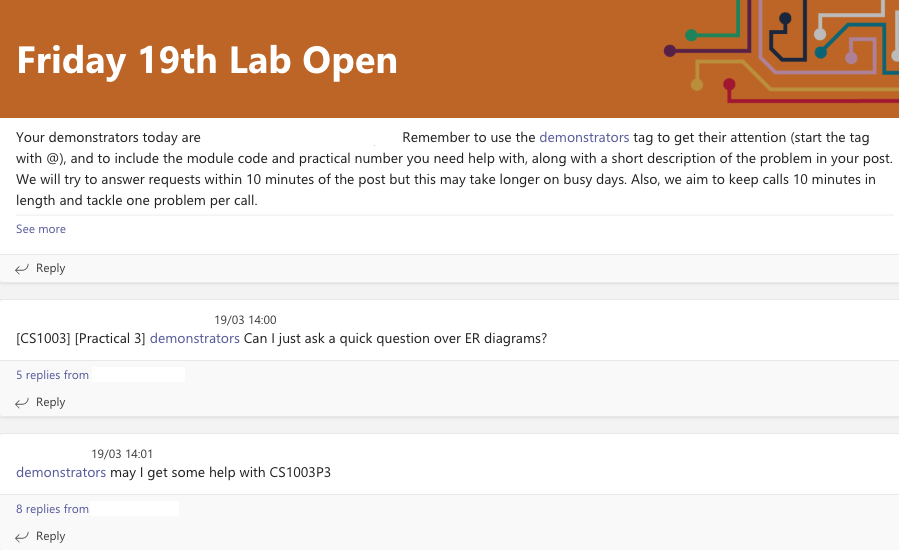
\includegraphics[width=\textwidth]{2context/images/teams1.png}
  \caption{An example of the first iteration process of managing online labs.}
\end{figure}

The second, and current, iteration of the current system uses a form input. This is accessed using a `Request Form' tab in the Microsoft Teams \cite{teams} CS1000 Labs team. 

\FloatBarrier
\begin{figure}[H]
  \centering
  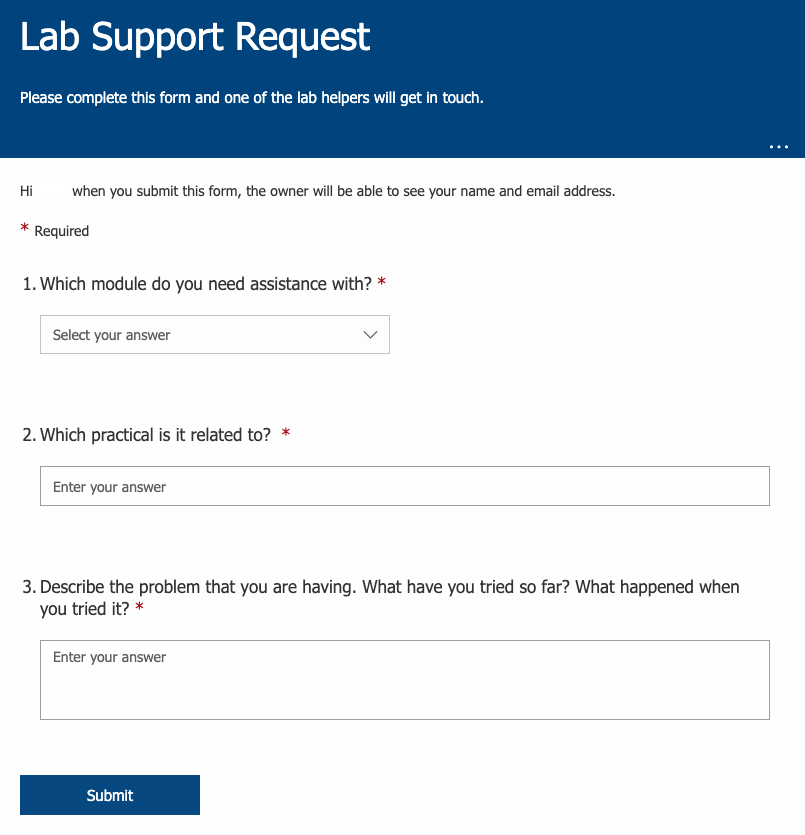
\includegraphics[width=0.85\textwidth]{2context/images/teams2a.png}
  \caption{The request form from the second iteration process of managing online labs.}
\end{figure}

The form uses Power Automate \cite{pauto} to post on a private demonstrator team channel (used only to create a notification for class demonstrators) and add the form data to a Microsoft List \cite{lists}.

\FloatBarrier
\begin{figure}[H]
  \centering
  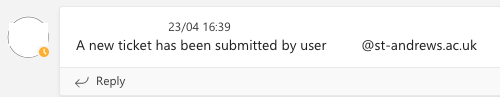
\includegraphics[width=0.6\textwidth]{2context/images/teams2b.png}
  \caption{The format of posts on the private demonstrator channel used to create notifications.}
\end{figure}

On this real-time collaborative spreadsheet, class demonstrators can assign themselves to students' requests before they make contact with the student through Microsoft Teams \cite{teams} or email (depending on the complexity of the issue). 

\FloatBarrier
\begin{figure}[H]
  \centering
  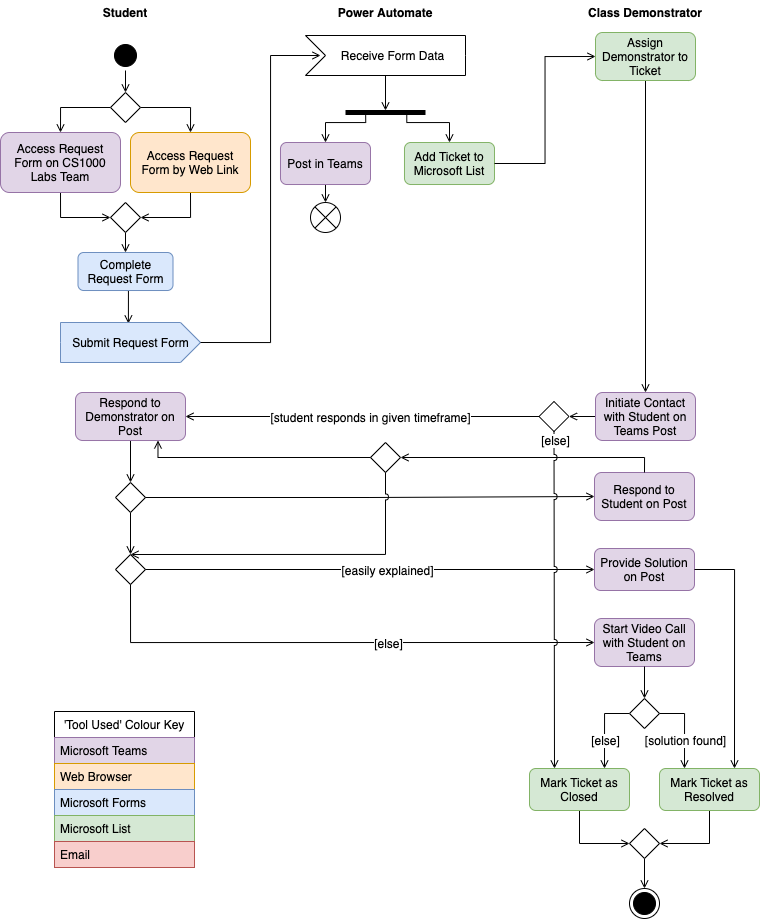
\includegraphics[width=\textwidth]{2context/images/activityRevised.png}
  \caption{\gls{uml} Activity diagram for existing method of managing student online lab request.}
\end{figure}

\newpage
\section{Classroom Management Tools}

ClassroomQ is a good example of existing classroom management tools. It offers a very simple system, where teachers can create a classroom which students can join, type a message and hit an `Assistance Needed' button to join the queue of students who need help. The basic process is shown below.

Firstly, the teachers start a classroom session.

\FloatBarrier
\begin{figure}[H]
  \centering
  
\includegraphics[width=0.5\textwidth]{2context/images/cq1.png}
  \caption{Teacher's screen when a class has not been started.}
\end{figure}

The classroom is created, showing the class code which students can use to join.

\FloatBarrier
\begin{figure}[H]
  \centering
  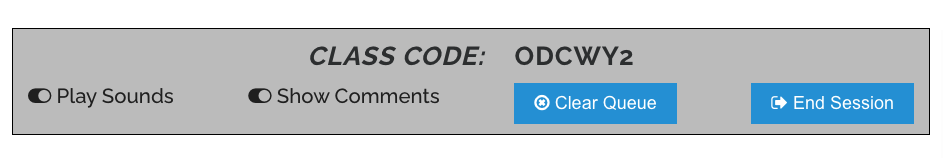
\includegraphics[width=0.75\textwidth]{2context/images/cq2.png}
  \caption{Real time classroom queue, showing class join code and current requests.}
\end{figure}

Students join by entering their name and class code.

\FloatBarrier
\begin{figure}[H]
  \centering
  
\includegraphics[width=0.5\textwidth]{2context/images/cq3.png}
  \caption{Student join page, showing sample class code and name.}
\end{figure}

Below is the image shown to students once they have joined the class. From this page they are able to type details of their problem in the comment section and then click the `Assistance Needed' button to join the queue.

\FloatBarrier
\begin{figure}[H]
  \centering
  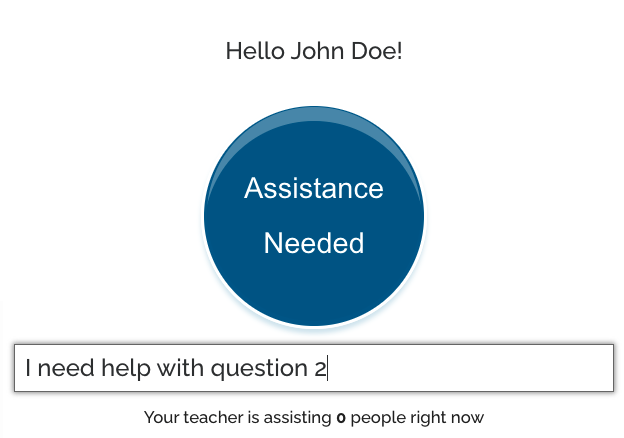
\includegraphics[width=0.5\textwidth]{2context/images/cq4.png}
  \caption{Student help request page.}
\end{figure}

Once the student has joined the queue, they are taken to the page below. This allows them to cancel their request as well as providing real time information about their position in the queue.

\FloatBarrier
\begin{figure}[H]
  \centering
  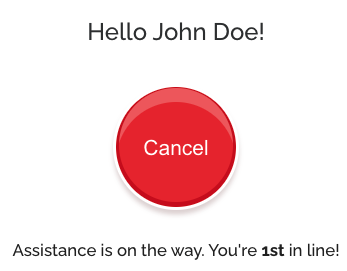
\includegraphics[width=0.5\textwidth]{2context/images/cq5.png}
  \caption{Student page after posting help request.}
\end{figure}

The teacher is then able to see an ordered view of the student's requests in on the class page.

\FloatBarrier
\begin{figure}[H]
  \centering
  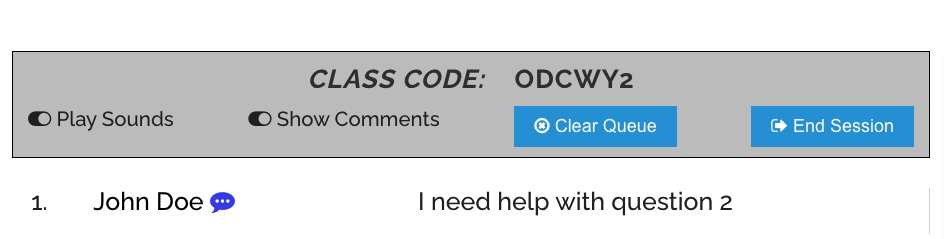
\includegraphics[width=0.75\textwidth]{2context/images/cq6.png}
  \caption{Teacher's class page view after the request has been posted.}
\end{figure}

\newpage
\section{Incident Management Tools}

Spiceworks Cloud Help Desk is a good example of existing incident management tools. It is a free to use, cloud-based help desk that is used by IT professionals. Traditionally, the system is used to track and manage IT issues in order to provide IT support, however the system could also be used to track and manage requests for help in our lab management domain. The basic process is shown below.

Firstly, students would access a link to the help portal and enter their email address.

\FloatBarrier
\begin{figure}[H]
  \centering
  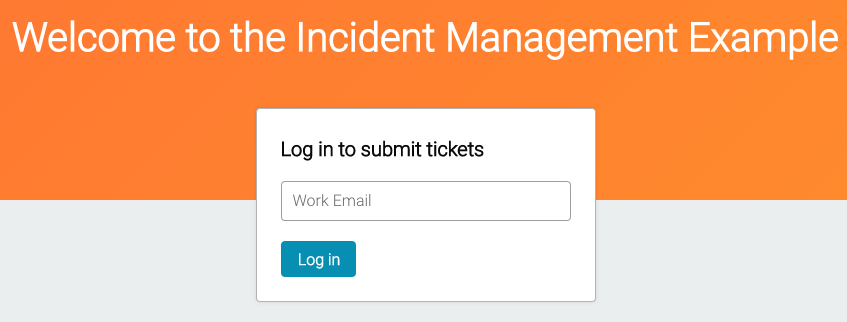
\includegraphics[width=0.5\textwidth]{2context/images/SWportalLogin.png}
  \caption{Login screen from portal link.}
\end{figure}

The student would then, if authorised, receive an email link to login to the portal. This would take them to the following form.

\FloatBarrier
\begin{figure}[H]
  \centering
  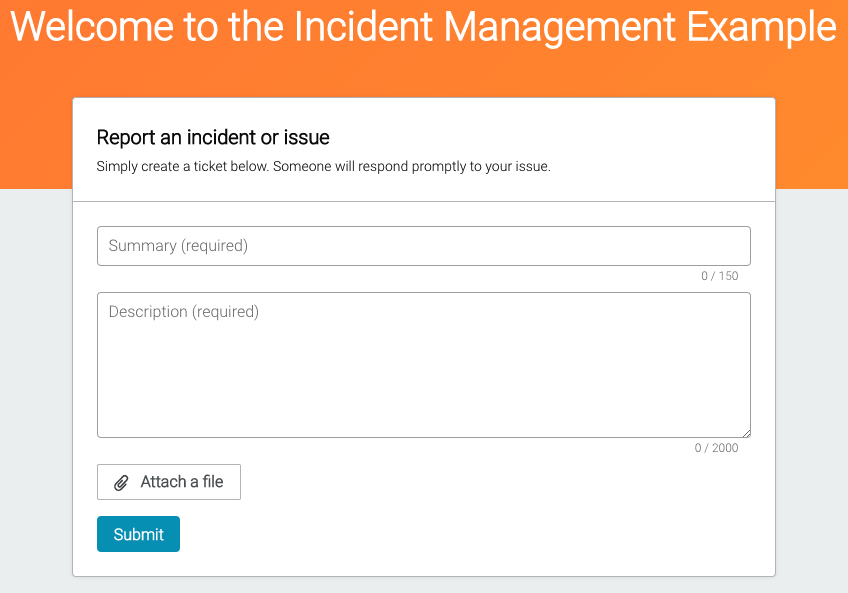
\includegraphics[width=0.65\textwidth]{2context/images/SWpostTicket.png}
  \caption{Ticket posting form, reached after login.}
\end{figure}

The ticket would then appear on the class demonstrator help desk.

\FloatBarrier
\begin{figure}[H]
  \centering
  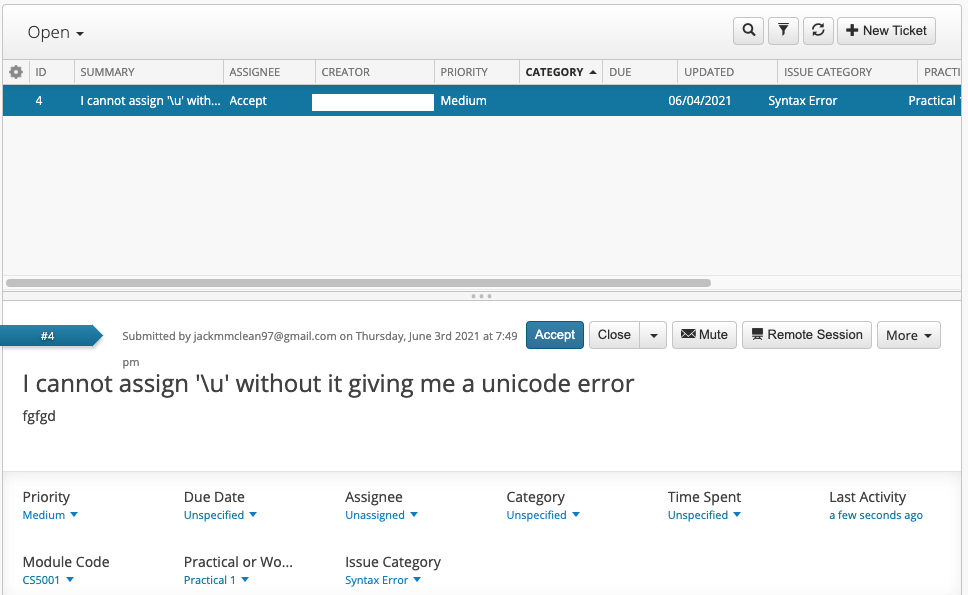
\includegraphics[width=0.85\textwidth]{2context/images/SWticketPage.png}
  \caption{The help desk ticket page, accessible to class demonstrators.}
\end{figure}

Class demonstrators are then able to respond to the ticket on Spiceworks, notifying the user by email, and initiate a video call on a different service if necessary. The demonstrator can then close the ticket when complete.

